\documentclass[17pt]{extarticle}

\usepackage{extsizes}

\usepackage[paperheight=9.6cm,paperwidth=17cm,margin=0.8cm]{geometry}
\parindent=0mm \parskip=3.2mm \linespread{1.15}

\usepackage{amsmath,amssymb,mathtools}
\usepackage{graphicx,xcolor,tikz}
\usetikzlibrary{positioning}
\usepackage[linguistics]{forest}
\usepackage{enumerate,enumitem}

\setlist{leftmargin=*}
\usepackage[russian]{babel}

% \definecolor{fon}{HTML}{0f1622}
% \definecolor{bluetri}{RGB}{45,155,190}
% \pagecolor{fon}
% \color{white}

\usepackage{mathspec}

\setmainfont[
	Path = f/,
	BoldFont=ib.ttf,
	ItalicFont=ii.ttf,
	BoldItalicFont=ibi.ttf
		]{i.ttf}
		
\setmathfont(Digits)[Path = f/]{i.ttf}
\setmathfont(Latin)[Path = f/]{ii.ttf}
\setmathfont(Greek)[Path = f/, Uppercase]{g.ttf}
\setmathfont(Greek)[Path = f/, Lowercase]{g.ttf}



\DeclarePairedDelimiter\lr{(}{)}
\newcommand{\newslide}[1]{\newpage \begin{center} \large #1
                          \end{center} \vspace{-5.5mm}}
\newcommand{\tr}[1]{\textcolor{red}{#1}}

\DeclareMathOperator{\rlbl}{relabel}
\DeclareMathOperator{\size}{size}
\DeclareMathOperator{\length}{length}
\DeclareMathOperator{\Rel}{Rel}
\DeclareMathOperator{\Rlbl}{Relabel}
\DeclareMathOperator{\Inse}{Insert}

\begin{document}

\ \\ [1cm]

\begin{center} {\Large Folding Polygons to Polyhedra} \bigskip \\
	{\large B. Zolotov, Ph.\,D. English Course} \end{center}

\newslide{Alexandrov's Theorem}

Is always brought up when it comes to gluing things. \medskip

If a gluing is homeomorphic to a sphere \\
and the sum of angles at each of \\
its vertices is $\le 360^\circ$\!, there $\exists\,!$ convex \\
polyhedron that corresponds to this gluing.

\newslide{Alexandrov's Theorem — Examples}

\begin{center}
	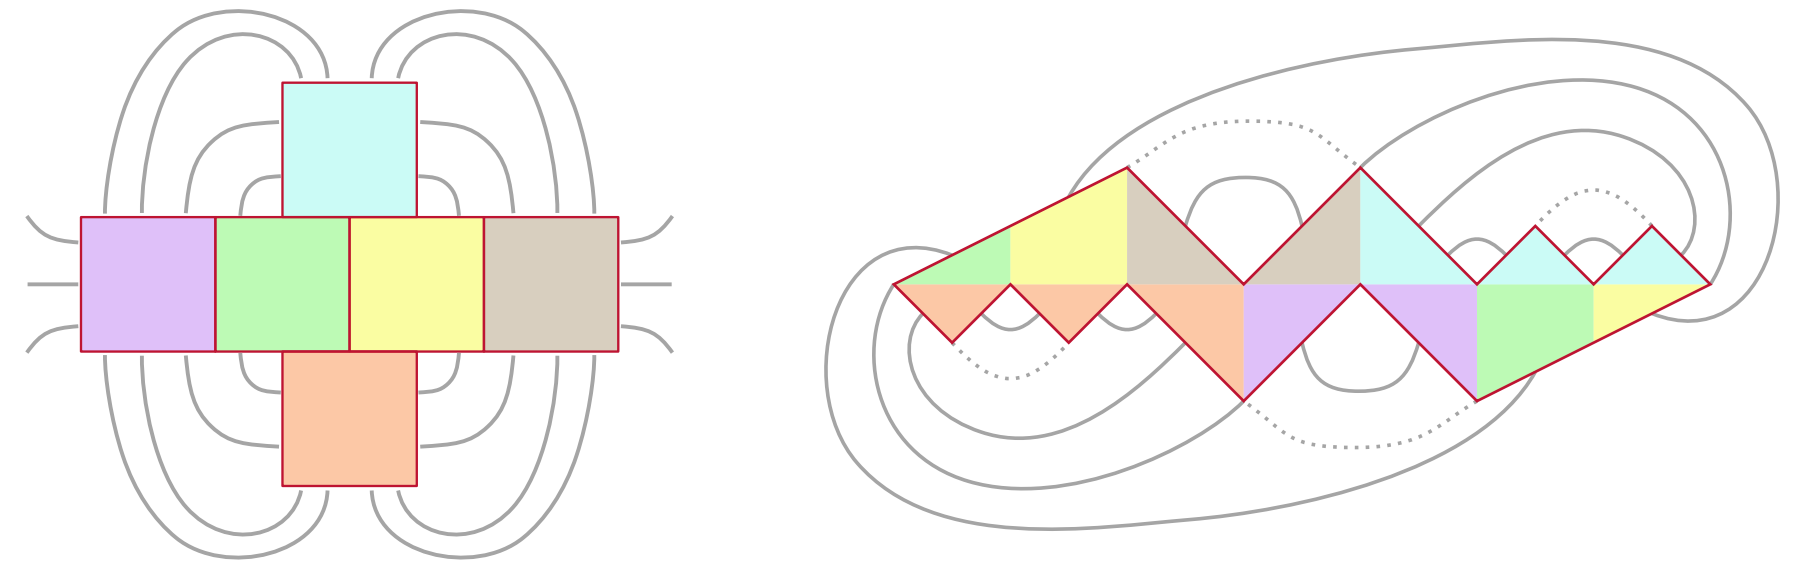
\includegraphics[width=0.6\textwidth]{minilec/alex-bef} \medskip \\
	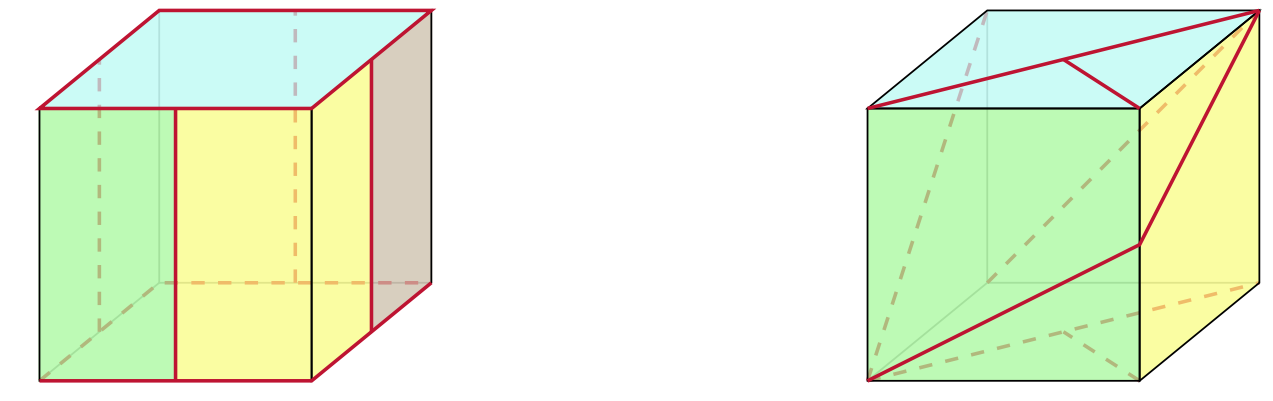
\includegraphics[width=0.6\textwidth]{minilec/alex-zaft}
\end{center}

\newslide{Folding a single polygon}

As we can see from the previous example, \\
a single polygon can be glued to itself, \\
the same conditions remain. \medskip \\
We will be {\it only} considering \\
foldability to {\it convex} polyhedra.

\newslide{A not-foldable polygon}

\begin{center}
	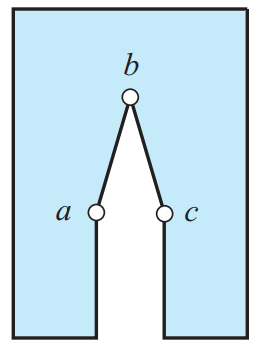
\includegraphics[width=3cm]{minilec/notf}
\end{center} \vspace{-5mm}

Consider where the reflex vertex can be glued?..

\newslide{Foldability of random polygons}

No matter how «a random polygon» is sampled, \\
we are expecting that it: \vspace{-4mm}

\begin{itemize}
	\item has at least two reflex vertices on average,
	\item the edge lengths are drawn from a \\
	cont. density distribution.
\end{itemize} \vspace{-4mm}

The probability that a random $n$-gon can be folded into a convex polyhedron approaches 0 as \(n \to \infty\).

\newslide{Perimeter-halving}

{\it Any convex} polygon can be folded into \\
a convex polyhedron by {\it perimeter halving.}

By varying the points half a perimeter apart we get \\
uncountably many {\it incongruent} polyhedra.

\newslide{Edge-to-edge folding}

Let us consider the subcase when entire edges \\
must be glued to entire edges.

There is a dynamic programming algorithm \\
to list all the gluings.

\newslide{Dynamic programming}

Idea: find a pair of matching edges, check angles, \\
reduce to two subproblems.

\begin{center}
	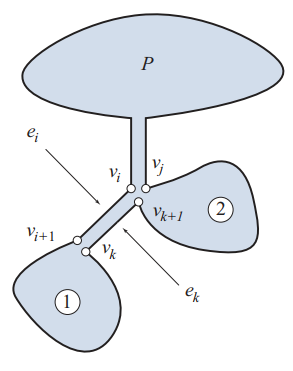
\includegraphics[width=3.2cm]{minilec/dynprog}
\end{center}

\newslide{All e2e gluings of the Latin cross}

\begin{center}
	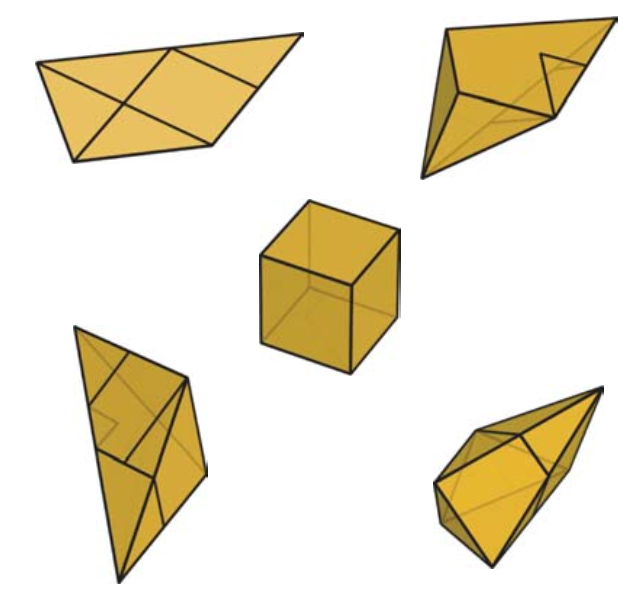
\includegraphics[width=7cm]{minilec/latincross}
\end{center}

\newslide{General algorithm} \vspace{-2mm}

There is also an algorithm that lists {\it all} the foldings; \\
it has exponential running time. \vspace{-5mm}

\begin{center}
	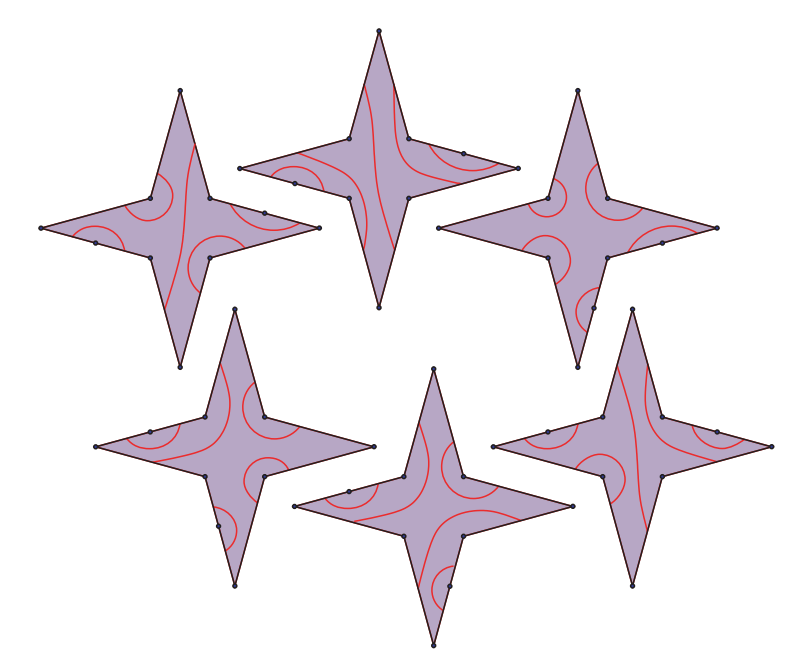
\includegraphics[height=5.3cm]{minilec/4star}
\end{center}

\newslide{Gluing tree} \vspace{-3mm}

Shows how the boundary of a folded polygon \\
corresponds to itself.\quad How to find the vertices \\
of the polyhedron by looking at \\
the vertices of the gluing tree?

\begin{center}
	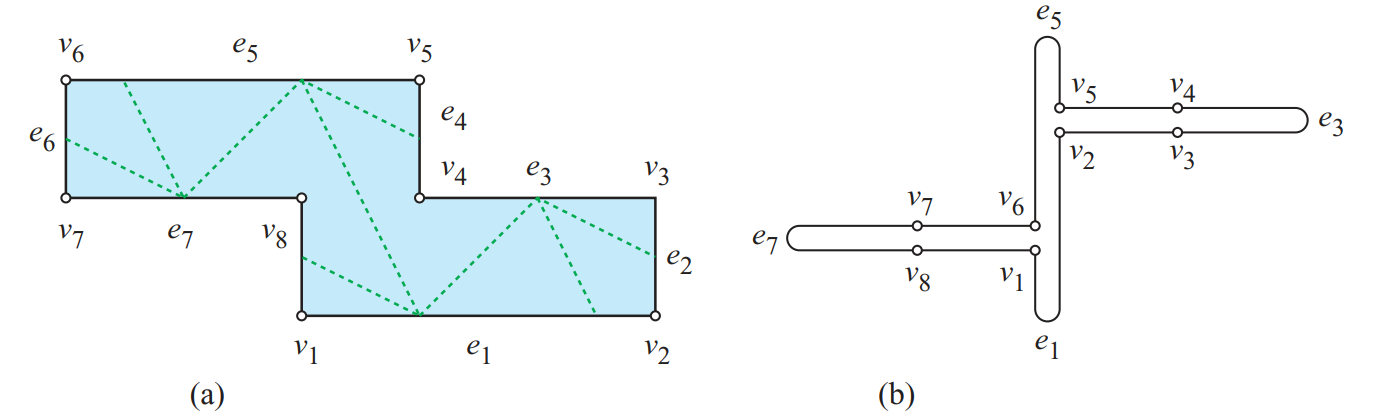
\includegraphics[height=3cm]{minilec/gtreerec}
\end{center}

\newslide{Analyse the curvature}
\begin{center}
	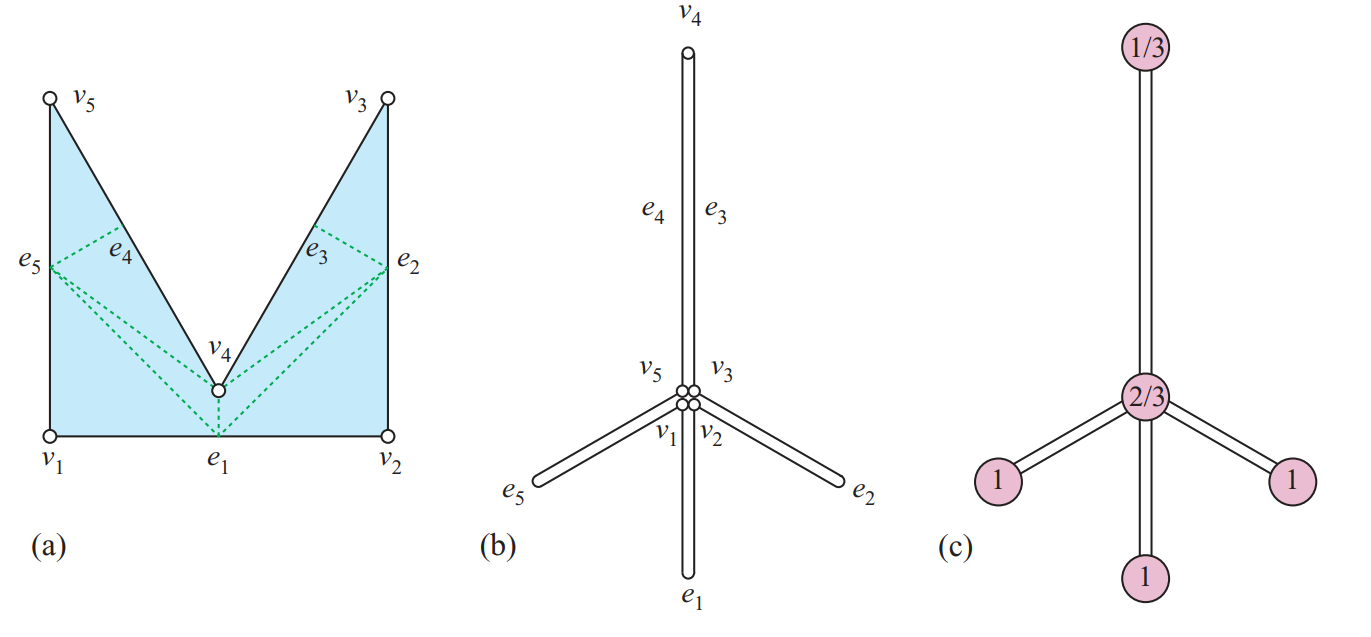
\includegraphics[height=5.2cm]{minilec/gtreecurv}
\end{center}

\newslide{Rolling belt}

A path in the gluing tree that: \vspace{-5mm}

\begin{itemize}
	\item Connects two leaves of the gluing tree \\
		that are either convex-vertex or \\
		fold-point leaves (positive deficit),
	\item The face angle to each side of the path is, \\
		at every point, convex.
\end{itemize}

\newslide{Rolling belts: examples}

Half of perimeter of any convex polygon or

\begin{center}
	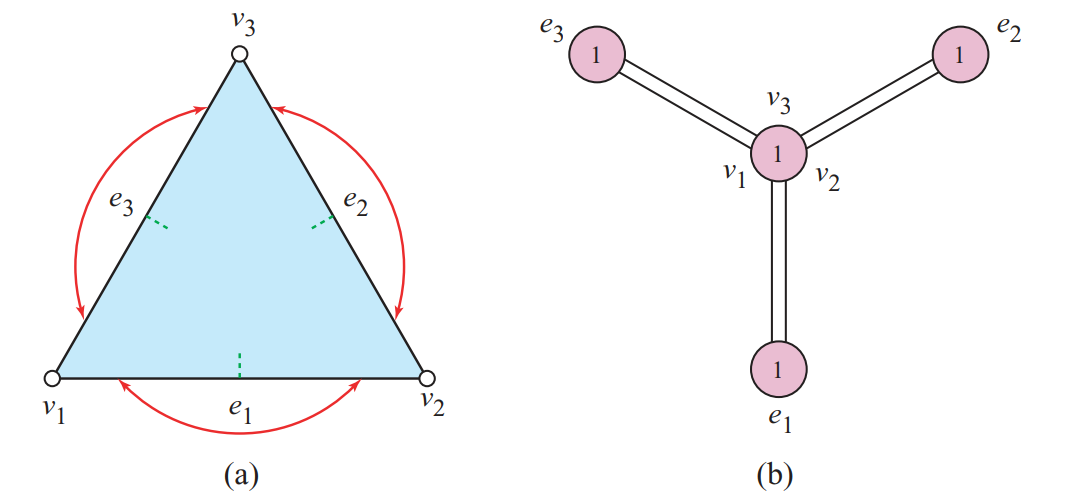
\includegraphics[height=4.5cm]{minilec/gtreerb}
\end{center}

\newslide{Gluing tree properties} \vspace{-5mm}

\begin{itemize}[itemsep=-3mm]
	\item Each leaf is either a vertex of the polygon, \\ or a fold point.
	\item At most one nonvertex may be glued at any \\ gluing-tree junction of degree \(d \ge 3\).
	\item A gluing tree may have at most two rolling belts \\ with distinct endpoints.
	\item The case of four fold-point leaves is possible \\ only under special circumstances.
\end{itemize}

\newslide{Rectangle with two rolling belts}

\begin{center}
	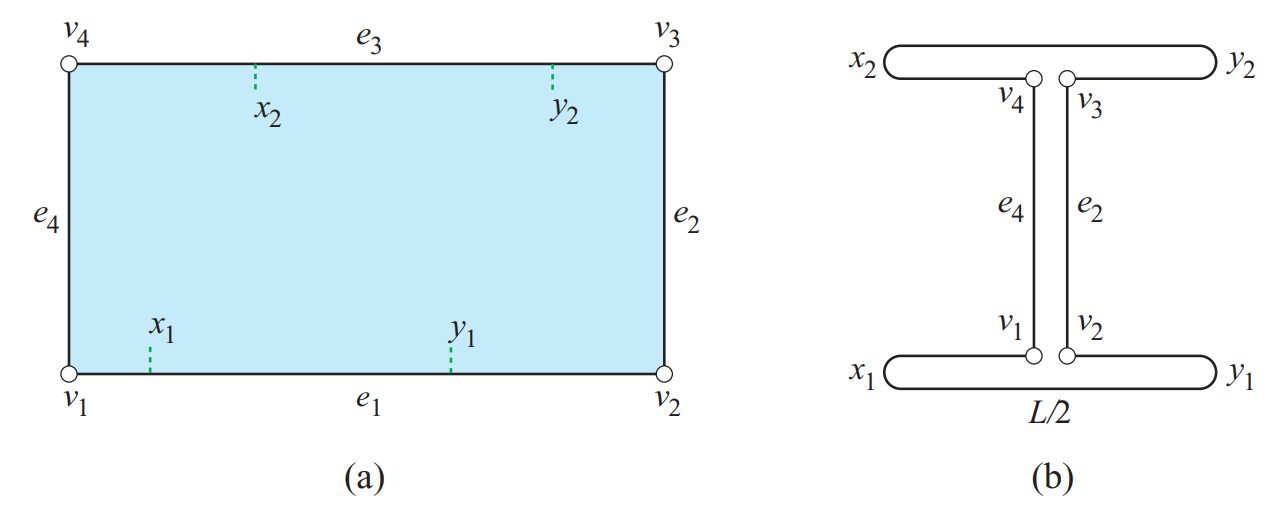
\includegraphics[height=5.3cm]{minilec/rectrb}
\end{center}

\newslide{Exponential number of gluing trees} \vspace{-2mm}

For any even \(n\), there is a polygon \(P\) of \(n\) vertices \\
that has \(2^{Ω(n)}\) combinatorially distinct \\
edge-to-edge Alexandrov gluings. \vspace{-2mm}

\begin{center}
	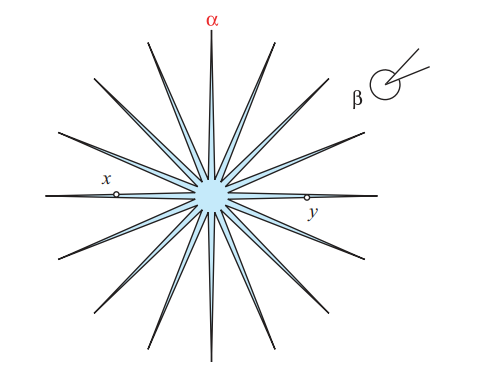
\includegraphics[width=5.1cm]{minilec/stargt}
\end{center}

\newslide{Contracted gluing trees}

There is the default gluing tree, it can be contracted in an exponential number of ways to form new trees.

\begin{center}
	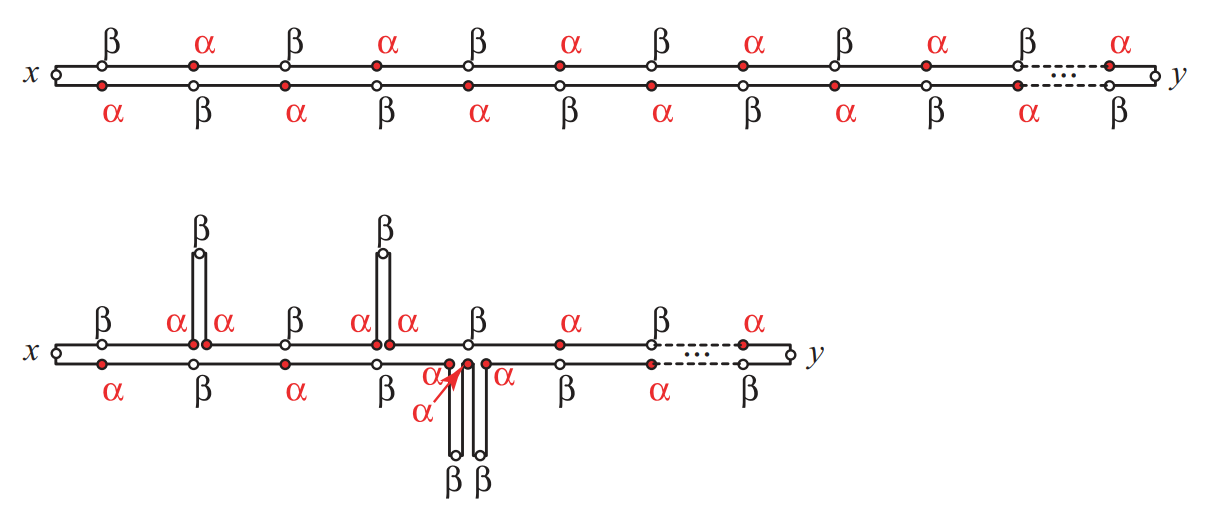
\includegraphics[height=4.5cm]{minilec/stargtcontract}
\end{center}

\newslide{Thank you for your attention!}

\begin{itemize}
	\item Not-foldable polygon, perimeter halving
	\item Algorithms listing foldings
	\item Gluing trees, rolling belts
	\item Exponentially many foldings
\end{itemize}

\end{document}
